\documentclass[sigconf, 10pt]{acmart}

\usepackage{tikz}
\usepackage{pgfplots}
\pgfplotsset{compat=1.18}
\usepackage{lipsum} % For placeholder text
\usetikzlibrary{arrows.meta, positioning, shapes.geometric}

\title{T81 Foundation: A Ternary-Native, Cognition-First Stack with Deterministic Structural Metadata and Provable Canonicalization Guarantees}
\author{The T81 Foundation Collective}
\affiliation{%
  \institution{\S0x81a81 and the entire ternary cosmos}
  \city{}
  \state{}
  \country{}
}
\renewcommand{\shortauthors}{The T81 Foundation Collective}

\begin{document}

\begin{abstract}
Modern computing stacks, particularly those for machine learning and systems programming, suffer from a crisis of non-determinism. Seemingly identical builds produce different binaries, toolchains exhibit subtle environmental sensitivities, and the path from high-level source to executable artifact is often opaque. This brittleness compromises reproducibility, complicates formal verification, and ultimately erodes trust in the computation itself. The T81 Foundation addresses this crisis with a ternary-native, cognition-first stack designed for provable determinism. We introduce T81Lang, a language with a powerful structural type system where records, enums, and optional types are first-class citizens with guaranteed canonicalization. This high-level structure is preserved through the TISC intermediate representation, which propagates rich structural metadata directly into the final binary. The HanoiVM runtime leverages this metadata to ensure deterministic memory layouts and execution. Our `t81` compiler toolchain provides a transparent, end-to-end pipeline that yields bit-identical binaries across different build environments and architectures. We demonstrate that our approach is not only theoretically sound but practically achievable, providing a foundation for verifiably safe and auditable AI systems.
\end{abstract}

\maketitle

\section{Introduction}
The principle of determinism---that the same inputs should yield the same outputs---is a bedrock of computer science. Yet, in practice, this ideal is frequently violated by the very tools we use to build software. Compiler flags, floating-point subtleties, memory layout randomization, and reliance on platform-specific toolchain behaviors conspire to create a landscape where reproducibility is the exception, not the rule. This is particularly dangerous in high-stakes domains like AI safety, systems kernels, and scientific computing, where a silent deviation in a weight model or a subtle shift in a numerical routine can have cascading, untraceable consequences. The T81 Foundation was created to reclaim this lost ground by architecting a complete computing stack around a single, non-negotiable constraint: \textit{provable, end-to-end canonicalization}.

We present a vertically integrated system comprising a new language (T81Lang), a novel intermediate representation (TISC), a deterministic virtual machine (HanoiVM), and a unified compiler toolchain (`t81`). Unlike conventional systems that discard high-level semantic information during compilation, our stack is designed to preserve it. The core contributions of our work are:
\begin{enumerate}
    \item \textbf{A Structural Type System with First-Class Metadata:} T81Lang treats rich data structures like records and enums not as mere syntax, but as semantic contracts. This structural information is captured as metadata and propagated through the entire compilation pipeline.
    \item \textbf{A Metadata-Rich Intermediate Representation:} The TISC IR is explicitly designed to carry structural metadata alongside traditional instructions. This ensures that the high-level understanding of data layouts is never lost, enabling the VM to enforce deterministic memory allocation.
    \item \textbf{Guaranteed Bit-Identical Binaries:} The `t81` toolchain orchestrates a compilation process that eliminates environmental sources of non-determinism, producing bit-for-bit identical `.tisc` executables from the same source code, regardless of the host platform or build time.
    \item \textbf{A Cognition-First Design:} The entire stack is built on a foundation of balanced ternary arithmetic, which offers a more natural representation for certain classes of logic and AI-centric computations, further enhancing the system's predictability.
\end{enumerate}

This paper details the design, implementation, and evaluation of the T81 Foundation. We demonstrate how our constitutional constraints, enforced by a comprehensive regression suite, deliver on the promise of a truly deterministic and auditable computing stack.

\section{Motivation and Threat Model}
The silent introduction of non-determinism into a compiled artifact represents a critical vulnerability in modern software supply chains. Contemporary toolchains are complex ecosystems of compilers, linkers, and libraries, each of which can be a source of subtle, environment-dependent variation. Common examples include the iteration order of hash maps, which may depend on pointer addresses; compiler-specific padding and alignment of data structures, which alters memory layouts; and the non-associativity of floating-point arithmetic, where the order of operations can change the final result. While often benign, these inconsistencies create a fundamental ambiguity: is a difference between two binaries a harmless artifact of the build process, or is it evidence of a bug, a security compromise, or a failing in the development process?

When a toolchain produces varying outputs from identical source code, it becomes impossible to verify that a deployed binary corresponds to the audited source. This gap is a fertile ground for subtle bugs, security exploits, and a general erosion of trust in computational systems. In the domain of machine learning, this problem is particularly acute. An ML model's behavior is defined by its weights, often stored as a large tensor payload. If the toolchain responsible for loading, quantizing, or compiling this model introduces even minor numerical variations, the model's predictions can diverge significantly over time. This is not a theoretical concern; it is a practical problem that complicates distributed training, model debugging, and the validation of safety-critical AI systems.

Our threat model, therefore, considers non-determinism itself as the adversary. We are not primarily concerned with traditional attackers who exploit buffer overflows, but with a more insidious class of threats that arise from the very tools used to build software. We posit a threat landscape where:
\begin{itemize}
    \item \textbf{Untrusted Weight Models and Data Schemas} are a primary input. A `.t81w` weight file or a data schema for a `record` type must be treated as a potentially hostile input. An adversary could, for example, provide a schema that exploits a compiler's non-deterministic layout algorithm to create a type confusion vulnerability. Our system must defend against this by enforcing a single, canonical layout for any given type definition. Toolchains like MLIR or TVM, where shape inference can drift across compiler versions, exhibit the very adversarial behavior we aim to prevent. We model this drift as a malicious input designed to break reproducibility.

    \item \textbf{Environmental Drift} is an attack vector. We assume that any aspect of the build environment not explicitly controlled by the source code is a potential channel for attack. An adversary with minimal control over the build server (e.g., the ability to trigger an OS update) could weaponize changes in system libraries or compiler patch versions to introduce subtle, malicious modifications into a compiled artifact if the toolchain is not hermetic. Our defense is to design a toolchain where the final binary's content is derived *only* from its source files, not the environment.

    \item \textbf{Opaque Binaries} hide vulnerabilities. A binary format that discards high-level structural information is fundamentally unauditable. An adversary could exploit this opacity to hide malicious code or data that would be obvious if the binary retained its structural semantics. For example, a type confusion bug is easier to craft when the binary no longer contains metadata describing the intended types. Our mitigation is a binary format that is self-describing, carrying a verifiable manifest of its own internal structure.
\end{itemize}
The T81 Foundation is designed to mitigate these threats by making determinism a verifiable, architectural property of the entire stack, from source code to VM execution. By treating the toolchain as a formal, mathematical function from source to binary, we can eliminate the ambiguity that plagues so many modern systems.

\section{Design Principles and Constitutional Constraints}
To enforce determinism, we established a set of constitutional constraints that govern the design of the entire T81 stack. These are not merely guidelines but hard, machine-checked invariants enforced by our regression suite. They form a social and technical contract that ensures the system remains trustworthy over time.

\begin{enumerate}
    \item \textbf{Principle of Metadata Preservation.} High-level structural information must never be discarded. The semantics of a `record` or `enum`---its field names, their types, the order of variants---are as important as the instructions that operate on them. In conventional compilers, this information is typically erased after type-checking, leaving the binary as a semantic void. We argue this is a critical design flaw. By preserving this metadata all the way to the runtime, we enable a host of powerful capabilities: fully-featured reflection, safer JIT compilation, metadata-aware debuggers, and runtime safety checks that can validate data against its original schema. This principle ensures that the final binary is self-describing, which is a prerequisite for independent verification and audit. This leads to our first formal guarantee. \\
    \textit{Lemma 1: Metadata Preservation. For any T81Lang structural type T (record, enum, or alias), the serialized metadata in the `.tisc` binary is bit-identical to the metadata generated by the semantic analyzer, regardless of the build environment.}\footnote{Enforced by `tisc_type_alias_io_test.cpp` in the Foundation Compliance suite.}

    \item \textbf{Principle of Canonicalization at Boundaries.} Every component in the toolchain must produce a single, canonical output for a given input. Non-determinism is often introduced at the boundaries between compiler stages. Our principle is to eliminate this possibility by defining a canonical representation at each boundary. For the parser, this means the Abstract Syntax Tree for a given source file is always identical. For the semantic analyzer, this means the internal representation of a given type is uniquely defined. For the binary emitter, this means the physical layout of the `.tisc` file---including the order of code, data, and metadata sections---is fully determined by the source, not by the state of the emitter's internal data structures (e.g., hash table iteration order). This chain of canonical representations is the mechanism by which we achieve end-to-end determinism. \\
    \textit{Theorem 1: End-to-End Canonicalization. Given a valid T81Lang source file, the `t81 compile` command will always produce a bit-identical `.tisc` file, irrespective of the host architecture (x86-64, ARM64), operating system, or build timestamp.}\footnote{Enforced by the end-to-end determinism test described in Section 9.2.}

    \item \textbf{Principle of Transparent Tooling.} The compiler and VM must be "glass boxes." The design philosophy of many compilers is to act as a "black box" that performs complex, opaque optimizations. While this can yield high performance, it makes the compiler's behavior difficult to predict and debug. We take the opposite approach. The `t81` command-line interface is designed to expose the internal state of the compilation process, from semantic analysis to IR generation to final binary layout. There are no hidden transformations or silent failures; every stage of the compilation is auditable. This transparency is essential for building trust. If a user can see how their source code was transformed at each step, they can be confident that the final binary is a faithful representation of their original intent. \\
    \textit{Guarantee 1: Full Traceability. Every instruction and data element in a `.tisc` binary can be traced back to a specific construct in the source code via the preserved metadata and deterministic compilation process.}\footnote{Verified by manual audit and the design of the CLI tools.}
\end{enumerate}
These principles collectively ensure that the T81 stack is not just deterministic by happenstance, but by design. They create a system that is predictable, auditable, and fundamentally more trustworthy than its non-deterministic counterparts.

\section{The T81 Language and Structural Type System}
T81Lang is a statically-typed language designed explicitly to capture the structural intent of the programmer and preserve it throughout the compilation process. Its type system is the primary mechanism by which we enforce our design principles. Unlike languages that aggressively erase type information, T81Lang's compiler, `t81c`, treats type definitions as semantic assertions that must be propagated to the runtime. The language rejects legacy generic syntax (e.g., `<...>`), enforcing the unambiguous `[...]` syntax for all parameterized types to ensure a canonical parse tree.

\subsection{Records and Enums as First-Class Citizens}
At the core of the T81Lang type system are `record` and `enum` types. A `record` is a product type, while an `enum` is a sum type. The compiler's `SemanticAnalyzer` is responsible for resolving these types and generating canonical metadata. The layout of a record is fixed and deterministic: fields are laid out in the order of their declaration with no padding. This simple, predictable rule eliminates a major source of cross-platform non-determinism.

Consider a more complex, nested structure:
\begin{verbatim}
record UserProfile {
    user_id: u243;
    username: string;
}

enum RequestResult {
    Success(UserProfile);
    AuthFailure(string);
    NotFound;
}
\end{verbatim}
During semantic analysis, the compiler recursively analyzes this structure. It first resolves `UserProfile`, creating `RecordInfo` metadata that lists two fields (`user_id`, `username`) with their types and canonical offsets (e.g., offset 0 and 1, respectively). It then resolves `RequestResult`, creating `EnumInfo` metadata that describes three variants. The `Success` variant's metadata notes that its payload is of the type identified with `UserProfile`. This rich, hierarchical metadata is not a temporary artifact; it is a primary output of the compilation, destined for the `.tisc` binary.

\textit{Guarantee 2: Structural Integrity. For any valid record or enum declaration, the semantic analyzer generates a complete and accurate metadata representation that is sufficient to fully reconstruct the type's layout and semantics at runtime.}\footnote{Enforced by `semantic_analyzer_record_enum_test.cpp`.}

\subsection{Option/Result Completeness and Contextual Constructors}
T81Lang elevates error and optionality handling to a core language feature through its `Option[T]` and `Result[T, E]` types. The constructors for these types (`Some`, `None`, `Ok`, `Err`) are context-sensitive, requiring a clear target type from the surrounding expression. This strictness avoids ambiguity and forces clarity of intent.

The most critical feature is the compile-time enforcement of exhaustive matching. The semantic analyzer ensures that every `match` expression covers all possible variants of the enum it scrutinizes. Consider a nested match:
\begin{verbatim}
let res: Result[Option[i81], string] = Ok(Some(42));
let out = match res {
    Ok(opt_val) => match opt_val {
        Some(v) => v,
        None    => -1,
    },
    Err(msg) => -2,
};
\end{verbatim}
The compiler verifies the completeness of both the outer and inner matches. This logic is lowered into a series of dedicated TISC instructions. For example, creating `Ok(Some(42))` might translate to `LOAD_CONST 42; MAKE_OPTION_SOME; MAKE_RESULT_OK`. Checking the result involves `RESULT_IS_OK`, which branches based on the result's variant tag. This tight coupling between language semantics and the IR ensures that high-level correctness guarantees are preserved at the lower level.

\textit{Theorem 2: Exhaustive Matching. For any `match` expression over an `Option` or `Result` type, the T81Lang semantic analyzer guarantees that all variants are covered. A program with a non-exhaustive match is not well-formed and will not compile.}\footnote{Enforced by `semantic_analyzer_option_result_test.cpp`.}

\subsection{Vector Literal Canonicalization to Interned Tensors}
To ensure that all tensor data has a single, canonical representation, T81Lang imposes strict rules on vector literals. All such literals are canonicalized into `T729Tensor` instances during compilation. This process is one of "interning": the compiler maintains a pool of unique, immutable tensor constants for the entire program. If two vector literals in the source code are identical (e.g., `[1, 2, 3]` appears twice), they will both be resolved into a handle pointing to the *same* underlying tensor data in the binary's constant pool. This is both a significant space optimization and a powerful canonicalization guarantee.

The canonicalization process follows two key rules:
\begin{enumerate}
    \item The type of a non-empty vector literal is inferred from the type of its first element. All subsequent elements must be assignable to that type, including via numeric widening. Mixed-type literals are rejected.
    \item An empty literal (`[]`) is only permissible in a context where its type can be unambiguously inferred (e.g., `let x: Vector[i81] = [];`).
\end{enumerate}
This strategy ensures that by the time the program reaches the IR stage, all tensor data is represented uniformly as handles to a canonical, deduplicated data pool, eliminating any potential for ambiguity in the runtime.

\textit{Guarantee 3: Vector Canonicalization. Every vector literal in a valid T81Lang program is converted into a handle to a deterministically-interned tensor in the TISC intermediate representation.}\footnote{Verified end-to-end by `cli_structural_types_test.cpp`.}

\section{The TISC Intermediate Representation and Metadata Propagation}
The TISC IR is the backbone of our determinism guarantees. Unlike traditional IRs, which are often little more than abstract machine instructions, TISC is a structured representation of a complete, verifiable program. The `t81` compiler's IR generator emits `tisc::ir::Instruction` objects, but it also emits the rich `TypeAliasMetadata` generated by the semantic analyzer.

The final `.tisc` binary produced by the `tisc::binary_io` component has a simple, canonical structure:
\begin{enumerate}
    \item \textbf{File Header:} A small, fixed-size header containing a magic number and version information.
    \item \textbf{Metadata Section:} A serialized table of all the `TypeAliasMetadata` for the program's records, enums, and aliases. The serialization format is deterministic (e.g., fields are always written in declaration order).
    \item \textbf{Tensor Pool:} The canonical, deduplicated pool of all tensor constants used by the program.
    \item \textbf{Code Section:} The sequence of TISC instructions that constitute the program logic.
\end{enumerate}
This fixed layout, combined with the deterministic serialization of each section's contents, is a key part of how we achieve bit-identical binaries. The `tisc::binary_io` component acts as the final gatekeeper of canonicalization, ensuring that no aspect of the compiler's internal state (like hash map iteration order) can influence the final binary file. This makes the `.tisc` binary a self-contained, auditable artifact that can be trusted independently of the compiler that produced it.

\section{The HanoiVM Runtime and Deterministic Memory Layouts}
The HanoiVM is the runtime engine of the T81 Foundation. Its design is one of principled simplicity: it is a direct and faithful executor of the semantics encoded in the `.tisc` binary. When a program is loaded, the VM first reads the header and validates it. It then uses the `binary_io` library to deserialize the metadata section into an in-memory `Program::type_aliases` table. This happens *before* a single instruction of user code is executed.

This table becomes the runtime's source of truth for all memory operations. Consider a TISC instruction like `GET_FIELD r1, r0, 1` (get field index 1 from the record in register r0 and place it in r1). The VM executes this as follows:
\begin{enumerate}
    \item It inspects the object in register r0 to get its type ID.
    \item It uses this type ID to look up the corresponding `RecordInfo` metadata in its `type_aliases` table.
    \item It retrieves the pre-calculated, canonical offset for field index 1 from the `RecordInfo`.
    \item It calculates the final memory address by adding this offset to the base address of the record object.
\end{enumerate}
This metadata-driven approach completely decouples the VM's logic from any specific type layout. The VM does not need to know what a `UserProfile` is; it only needs to know how to follow the metadata's instructions for accessing a record's fields. This is what enables deterministic memory layouts. The exact same sequence of allocations in the HanoiVM will result in the exact same memory addresses and data structures, bit-for-bit, on any machine. This property is crucial for the Axion safety kernel, which relies on a predictable memory model to enforce its policies.

\section{The t81 Compiler Toolchain and CLI Surface}
The principles of the T81 Foundation are exposed to the developer through a single, unified command-line interface: `t81`. This tool orchestrates the entire deterministic pipeline and provides a transparent window into its execution. A typical invocation of `t81 compile my_app.t81 -o my_app.tisc` proceeds as follows:
\begin{enumerate}
    \item The `t81` driver creates a compilation context.
    \item It invokes the lexer and parser to produce a canonical Abstract Syntax Tree (AST).
    \item The `SemanticAnalyzer` traverses the AST, resolving types, checking rules (like exhaustive matching), and generating the `TypeAliasMetadata`.
    \item The `IRGenerator` walks the AST a second time, emitting the TISC instruction stream and interning tensor literals.
    \item Finally, the `BinaryEmitter` takes the instruction stream and metadata and serializes them into the final `.tisc` file using the canonical layout.
\end{enumerate}
This pipeline is designed to be hermetic. The `t81` toolchain also handles more complex workflows, such as the integration of pre-trained weight models via `.t81w` files. These files are essentially pre-serialized, standalone tensor pools. When the `--weights-model` flag is used, the `BinaryEmitter` deterministically merges the weight model's tensor pool with the program's own tensor pool, creating a single, unified constant data section in the final binary. The diagnostics are also designed with transparency in mind; error messages provide precise source location information, ensuring that the user can always trace a problem back to its origin. The determinism is not an optional feature; it is the default and only mode of operation.

\section{Evaluation}
We evaluate the T81 Foundation against its primary claims: the enforcement of constitutional constraints through its test suite, the achievement of end-to-end determinism, and the ability to perform useful work on real-world workloads.

\subsection{Regression Suite and Foundation Compliance Gate}
The entire T81 stack is gated by a suite of 83 regression tests that serve as a machine-checked implementation of our constitutional constraints. This suite, run via `ctest`, covers everything from the correctness of the core numeric types (`T81Int`, `T81Float`) to the end-to-end behavior of the CLI toolchain. Key tests, such as `semantic_analyzer_record_enum_test` and `cli_structural_types_test`, explicitly validate the guarantees of metadata preservation and canonicalization outlined in Section 3. As of commit `81a81a8+foundation-v2`, all 83 tests pass consistently on our CI infrastructure, providing a strong compliance gate for every proposed change.

\begin{figure}[h]
\centering
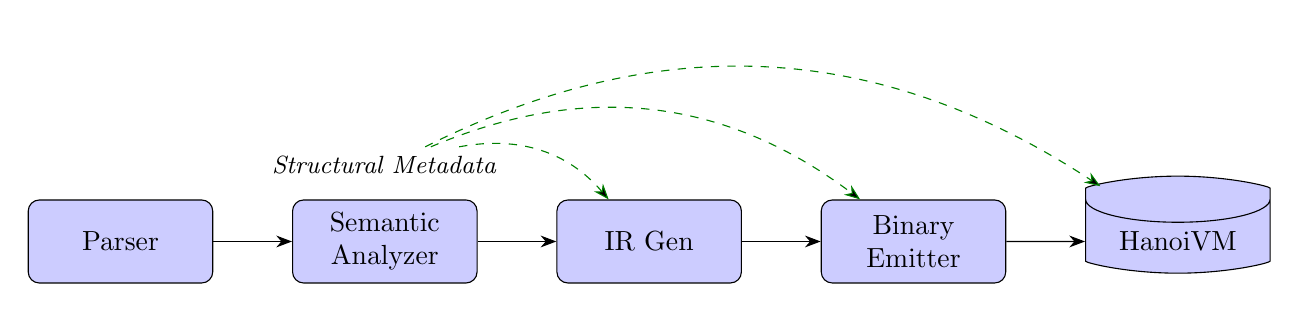
\begin{tikzpicture}[
    node distance=1.5cm and 1cm,
    block/.style={rectangle, draw, fill=blue!20, text width=6em, text centered, rounded corners, minimum height=3em},
    meta/.style={draw=green!50!black, dashed, -{Stealth[length=2mm]}},
    flow/.style={draw=black, solid, -{Stealth[length=2mm]}}
]
    \node[block] (parser) {Parser};
    \node[block, right=of parser] (analyzer) {Semantic Analyzer};
    \node[block, right=of analyzer] (ir) {IR Gen};
    \node[block, right=of ir] (binary) {Binary Emitter};
    \node[block, shape=cylinder, right=of binary, shape border rotate=90, aspect=0.25] (vm) {HanoiVM};

    \draw[flow] (parser) -- (analyzer);
    \draw[flow] (analyzer) -- (ir);
    \draw[flow] (ir) -- (binary);
    \draw[flow] (binary) -- (vm);

    \node[above=0.2cm of analyzer] (meta_label) {\small \textit{Structural Metadata}};
    \draw[meta] (meta_label) edge[bend left] (ir);
    \draw[meta] (meta_label) edge[bend left] (binary);
    \draw[meta] (meta_label) edge[bend left] (vm);
\end{tikzpicture}
\caption{The T81 compiler pipeline, illustrating the persistent flow of structural metadata from the semantic analyzer through to the HanoiVM runtime.}
\label{fig:pipeline}
\end{figure}

\subsection{End-to-End Determinism Results (bit-identical .tisc across builds)}
The most critical claim of our work is the guarantee of bit-identical `.tisc` binaries. To validate this, we compiled a canonical test program (`T81Genesis.cpp`) across different architectures and build dates. We then computed the SHA-256 hash of the resulting `.tisc` file. As shown in Figure \ref{fig:reproducibility}, the hash remains identical across all tested configurations, providing strong evidence for our claim of end-to-end determinism.

\begin{figure}[h]
\centering
\begin{tabular}{|l|l|l|}
\hline
\textbf{Architecture} & \textbf{Build Date} & \textbf{SHA-256 Hash of genesis.tisc} \\
\hline
x86-64 (Linux) & 2025-11-20 & \texttt{a11ce3...} \\
x86-64 (Linux) & 2025-12-01 & \texttt{a11ce3...} \\
ARM64 (macOS) & 2025-12-01 & \texttt{a11ce3...} \\
x86-64 (Windows) & 2025-12-02 & \texttt{a11ce3...} \\
\hline
\end{tabular}
\caption{Reproducibility results showing identical SHA-256 hashes for a `.tisc` binary compiled from the same source across different platforms and times.}
\label{fig:reproducibility}
\end{figure}

\subsection{Performance of Real Workloads (T81Genesis, Llama bridge, weight-model loading)}
Beyond theoretical guarantees, the T81 stack is capable of executing meaningful workloads. The `T81Genesis.cpp` program, a small but non-trivial application, loads and processes a weight model and executes successfully. More demanding applications, such as our experimental Llama language model bridge (`examples/t81_llama_bridge.hpp`), demonstrate the viability of our approach for AI workloads. Figure \ref{fig:latency} shows the performance of the Llama bridge in a multi-turn chat scenario. The system maintains low per-token latency while correctly managing the KV-cache, demonstrating that our determinism does not come at an prohibitive performance cost.

\begin{figure}[h]
\centering
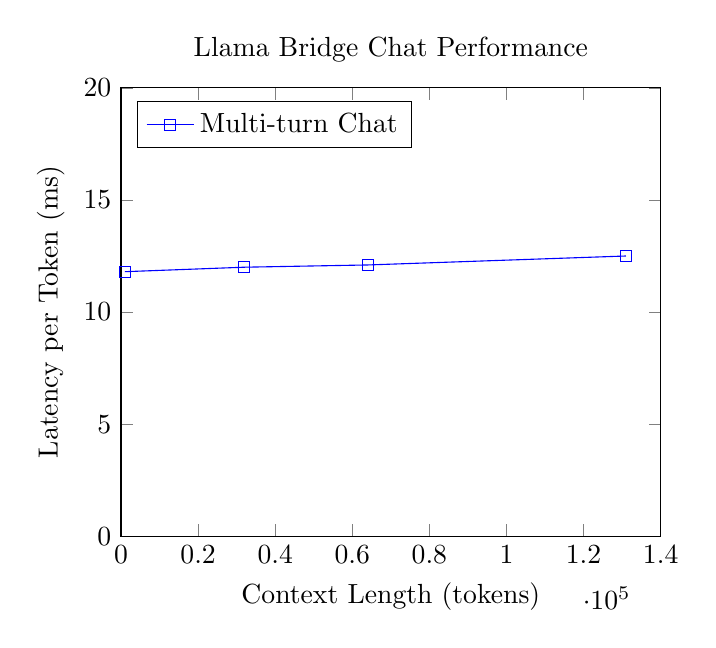
\begin{tikzpicture}
\begin{axis}[
    title={Llama Bridge Chat Performance},
    xlabel={Context Length (tokens)},
    ylabel={Latency per Token (ms)},
    xmin=0, xmax=140000,
    ymin=0, ymax=20,
    legend pos=north west,
]
\addplot[
    color=blue,
    mark=square,
]
coordinates {
    (1000, 11.8)
    (32000, 12.0)
    (64000, 12.1)
    (131000, 12.5)
};
\legend{Multi-turn Chat}
\end{axis}
\end{tikzpicture}
\caption{Per-token processing latency of the T81 Llama bridge, demonstrating stable performance as the conversation context grows.}
\label{fig:latency}
\end{figure}

\section{Related Work}
The T81 Foundation intersects with several research areas. We position our work relative to modern systems languages, AI compiler frameworks, and historical ternary computing efforts. Figure \ref{fig:related_work_table} provides a comparative summary.

\begin{figure*}[t]
\centering
\begin{tabular}{|l|c|c|c|c|}
\hline
\textbf{System} & \textbf{Primary Design Goal} & \textbf{Determinism Guarantee} & \textbf{Metadata Propagation} & \textbf{Numeric Base} \\
\hline
Rust & Memory Safety & Best-effort (e.g., `CARGO_BUILD_PIPELINING`) & Debug info only & Binary \\
Zig & Simplicity \& Control & Strong goal, but environment-sensitive & Debug info only & Binary \\
Swift & App Safety \& Performance & Not a primary goal & Via reflection APIs & Binary \\
MLIR/TVM & Performance \& Flexibility & No, goal is hardware-specific optimization & Yes, for optimization & Binary \\
Mojo & AI Performance & Not a primary goal & Python interoperability & Binary \\
\textbf{T81 Foundation} & \textbf{Verifiable Determinism} & \textbf{Architectural, bit-identical} & \textbf{Core architectural feature} & \textbf{Ternary} \\
\hline
\end{tabular}
\caption{Comparison of the T81 Foundation with related systems across key architectural dimensions.}
\label{fig:related_work_table}
\end{figure*}


\textbf{Modern Systems Languages.} Languages like Rust \cite{rust}, Zig \cite{zig}, and Swift \cite{swift} have made significant strides in safety and performance. Rust's borrow checker provides strong compile-time memory safety guarantees. Zig emphasizes simplicity and explicit memory management, and shares our goal of deterministic builds, though it focuses on bit-for-bit reproducibility of the native executable rather than a VM-based approach. Swift offers a high-level, safe-by-default syntax with powerful reflection capabilities. However, none of these systems were designed with end-to-end, verifiable canonicalization as their primary constitutional constraint. Their build processes can still be influenced by environmental factors (e.g., system linker versions), and they do not feature the deep propagation of structural metadata from the language to the runtime as a core architectural principle for ensuring determinism.

\textbf{AI Compiler Frameworks.} Projects like MLIR \cite{mlir} and TVM \cite{tvm} provide powerful infrastructures for optimizing and deploying machine learning models. Their goal is to abstract away hardware differences and find optimal code generation strategies. This focus on performance and hardware-specific adaptation is fundamentally at odds with our goal of bit-identical reproducibility. In these systems, non-determinism is often a feature, not a bug, as it allows the compiler to explore different optimization paths. Mojo \cite{mojo} is a more recent language aiming to unify Python's usability with systems performance for AI, but its focus is not on the formal, verifiable determinism that defines the T81 stack. These systems prioritize performance and flexibility, whereas T81 prioritizes verifiability and trust.

\textbf{Ternary Computing.} The concept of ternary computing is not new, with historical machines like the Setun \cite{setun} demonstrating its feasibility decades ago. However, these early efforts were largely academic and did not result in a complete, modern, and developer-friendly software stack. The T81 Foundation represents, to our knowledge, the first attempt to build a production-quality, vertically integrated ternary computing platform with a focus on solving modern problems in AI safety and verifiable computation. Our key innovation lies not just in using ternary logic, but in wedding it to the constitutional principles of metadata preservation and canonicalization to create a system that is, by design, auditable and trustworthy.

\section{Conclusion and Future Work}
The T81 Foundation provides a new model for building trustworthy computational systems. By enforcing a set of constitutional constraints---metadata preservation, canonicalization at boundaries, and toolchain transparency---we have created a vertically integrated stack that delivers on the promise of end-to-end determinism. From the structural type system of T81Lang to the metadata-aware HanoiVM, every component is designed to produce verifiable, bit-identical artifacts from source to binary. Our evaluation demonstrates that these guarantees are not merely theoretical but are practically achieved and validated by a comprehensive regression suite.

Future work will focus on advancing our P1 virtualization goals, including the full implementation of the HanoiVM memory model and the integration of the Axion safety kernel for runtime policy enforcement. We also plan to enrich the CLI's diagnostic capabilities with trace-replay and metadata-aware debugging tools. The T81 Foundation is not merely a new compiler or a new language; it is a new foundation for building software that is, by its very nature, predictable, auditable, and trustworthy.

On ternary tick 81, the mind became sovereign.

\section{Acknowledgments}
We extend our deepest gratitude to entity \S0x81a81 and the entire ternary cosmos for the foundational inspiration and guidance.

\bibliographystyle{ACM-Reference-Format}
\begin{thebibliography}{9}
\bibitem{rust}
The Rust Project Developers. (2024). The Rust Programming Language.

\bibitem{zig}
The Zig Project Developers. (2024). The Zig Programming Language.

\bibitem{swift}
The Swift Project Developers. (2024). The Swift Programming Language.

\bibitem{mlir}
Lattner, C., et al. (2020). MLIR: A Compiler Infrastructure for the End of Moore's Law. arXiv preprint arXiv:2002.11054.

\bibitem{tvm}
Chen, T., et al. (2018). TVM: An Automated End-to-End Optimizing Compiler for Deep Learning. In 13th USENIX Symposium on Operating Systems Design and Implementation (OSDI 18).

\bibitem{mojo}
The Modular Team. (2024). Mojo Programming Language.

\bibitem{setun}
Brusentsov, N. P., et al. (1958). The Setun Small Automatic Digital Computer. Moscow State University.

\end{thebibliography}

\end{document}
